%%%% CHARACTERIZATION OF EXTRAPOLATION TECHNIQUES %%%%
\chapter{Performance errors incurred by linear extrapolation methods}\label{chap:07_Characterization_Extrapolation}
In this chapter, we evaluate, through a comprehensive set of the numerical simulations described in \chapref{chap:06_Simulation_Framework}, the performance of two extrapolation-based navigational methods.
The methods considered here are chosen for their broad applicability to arbitrary sound fields due to the linear nature of the processing involved.
However, these methods are also susceptible to violating the region of validity restriction (see \secref{sec:02_Acoustical_Theory:Helmholtz_Equation}) if the listener attempts to navigate beyond the distance of the nearest source to the microphone.
Through the analyses presented here, we aim to determine, in terms of the metrics enumerated in \secref{sec:06_Simulation_Framework:Metrics}, the nature and degree of any penalties incurred by violating this region of validity restriction.

%% saved for a paper abstract
%In the first method, a plane-wave decomposition is employed to simplify the translation operation, however different methods and grid distributions for the plane-wave decomposition can introduce varying errors.
%Consequently, these parameters are first explored in isolation via numerical simulations of a single-microphone array, as described in \chapref{chap:06_Simulation_Framework}.
%Results show that matching the number of plane-waves to the number of ambisonics signals and employing the ``beamforming'' plane-wave decomposition method yields the most reliable results.
%%NOTE%% for the paper, make sure we establish right away the universality of this paper in that it should apply to all linear methods

%The second navigational method employs spherical harmonic translation coefficients to directly extrapolate the ambisonics signals.
%Performance errors are characterized for both methods via numerical simulations in terms of the metrics identified in \secref{sec:06_Simulation_Framework:Metrics}.
%Results show that both methods tend to exhibit two distinct regimes of behavior for far- and near-field sources, and that the performance for near-field sources is often degraded (compared to that for far-field sources) due to the violation of the region of validity restriction.
%In particular, both methods were found to incur significant errors in both overall level and localization when the region of validity restriction is violated.
%Additionally, the plane-wave translation method is shown to perform well for far-field sources, whereas the ambisonics translation method yields significant errors which tend to increase steadily with navigation distance.

\section{Introduction}\label{sec:07_Characterization_Extrapolation:Introduction}
According to ambisonics theory (reviewed in \secref{sec:02_Acoustical_Theory:Helmholtz_Equation}), an ambisonics recording of a sound field contains information about the spatial and temporal distribution of sound over the entire spherical free-field region surrounding the microphone (i.e., the so-called \textit{region of validity}) \citep{Williams1999,GumerovDuraiswami2005,Zotter2009PhD}.
However, recall that a finite-order expansion of a sound field yields only an approximation to that sound field, the accuracy of which decreases with increasing frequency and distance from the expansion center \citep{Poletti2005,WardAbhayapala2001} (see \eqnref{eq:01_Introduction:kr_Inequality}), so the prospect of navigating such a sound field is inherently limited.
Fortunately, this limitation is primarily a technical one, since synthetic sound fields can be generated to arbitrarily high orders and microphone array technology%
\footnote{See, for example: the Zylia ZM-1 \citep{ZyliaZM1URL}, the mh acoustics Eigenmike \citep{EigenmikeURL}, and the VisiSonics Audio Camera \citep{VisiSonicsAudioCameraURL}.}
is rapidly advancing such that it may soon be practical to capture very high-order expansions of real sound fields.

The more fundamental limitation of the spherical-harmonic description of sound fields is that the region over which the expansion is valid is limited by the nearest sound source (or scattering body) to the expansion center (as discussed in \secref{sec:02_Acoustical_Theory:Helmholtz_Equation}).
Consequently, near-field sources pose a particularly limiting problem to navigation.
The precise consequences of violating this region of validity restriction have not been clearly determined, and are a primary focus of this chapter.

Several previous studies have developed extrapolation-based navigational methods from a single ambisonics microphone.
In the following section, we provide a critical review of these existing methods and identify the main challenges they face.
All of the methods discussed below are listed in \tabref{tab:01_Introduction:Methods}.

%% PREVIOUS WORK %%
\subsection{Previous work}\label{sec:07_Characterization_Extrapolation:Previous_Work}
Perhaps the most intuitive navigational method is the \textit{virtual ambisonics} method, as described in \secref{sec:03_Navigation_Techniques:VA_Technique}.
In this method, the ambisonics signals are first decoded for a given loudspeaker array, which is then simulated in a virtual space with the listener at any desired position within the array.
The combined signals arriving at the virtual listener from the virtual loudspeaker array are then computed numerically and played back to the real listener.
Some advantages of this method are that we are free of the practical limitations (such as space, floors/walls, cost, etc.) common to physical loudspeaker arrays and that we can leverage the wealth of experience with real ambisonics systems that has been accumulated by researchers in this field.

For example, \citet{Frank2008} showed that so-called ``max-$r_{\textrm{E}}$'' decoding schemes yield more accurate localization at off-center positions and \citet{Satongar2013b} showed that off-center localization improves with increasing ambisonics expansion order.
Also, to account for the finite distances of loudspeakers from the listening position, \citet{Daniel2003b} developed a near-field-compensated decoding scheme which treats the loudspeakers as point-sources and consequently reconstructs the sound field more accurately at off-center locations.

As it has been defined, this method has no knowledge of any source (or obstacle) positions; consequently, depending on the positions of any sources in the sound field, the listener may inadvertently navigate too far such that the region of validity restriction is violated.
This method also inherently introduces a limit on the navigable region of the listener due to the finite size of the virtual array.
Although it remains unclear in what way the performance may degrade if the listener navigates outside the virtual array, the issue would be avoided entirely if plane-wave sources were used, as done in the plane-wave translation method (described in \secref{sec:03_Navigation_Techniques:PW_Technique}).

The \textit{plane-wave translation} method entails computing a plane-wave expansion of the sound field and translating along each plane-wave term.
\citet{MenziesAlAkaidi2007b} first derived the mathematical operations required for this method, although they did so while developing a technique to more accurately render synthetic near-field sources binaurally by way of a plane-wave expansion and translation.
\citet{SchultzSpors2013} later formulated the plane-wave translation method for the purpose of sound field navigation and examined the time- and frequency-domain consequences of the translation operation.
Similar to the virtual ambisonics method described above, this method is also prone to violating the region of validity restriction in the presence of near-field sources.

\citet{HahnSpors2015b} evaluated spectral coloration induced by the method by visually examining impulse and frequency responses and found that the induced coloration is often mitigated by matching $Q$, the number of plane-wave terms, to $N$, the number of ambisonics signals (i.e., the so-called ``critically-sampled'' condition, when $Q = N$) \citep[section 5]{HahnSpors2015b}. % ``friendly aliasing''
In the same study, the authors found that when $Q > N$ (in the so-called ``oversampled'' condition), navigating parallel to the direction of a source introduced less coloration than navigating perpendicularly. % only true in oversampling conditions
The localization properties of this method were explored by \citet{Winter2014}, who showed that the range over which accurate localization is achieved increases with ambisonics expansion order and that increasing the number of plane-wave-expansion terms beyond critically-sampled does not improve localization.
More recently, \citet{TylkaChoueiri2015} evaluated the localization errors using the velocity and energy localization vectors developed by \citet{Gerzon1992}, although the perceptual relevance of the findings of this study are limited since the analysis does not take into account the precedence effect.

Another navigational method, referred to here as \textit{ambisonics translation} and described in \secref{sec:03_Navigation_Techniques:SR_Technique}, is to translate the ambisonics expansion center by re-expanding the sound field about the desired point.%
\footnote{Relatedly, \citet{AhrensSpors2009} proposed a method which uses very similar mathematical operations (Bessel function translations) in order to analytically move in two dimensions the ``sweet-spot'' within a circular loudspeaker array.}
\citet{GumerovDuraiswami2005} derived recurrence relations which enable fast computation of such re-expansions and \citet{Zotter2009PhD} extended those derivations to real-valued spherical harmonics.
A subset of these derivations are replicated in \apxref{chap:A1_Navigation_Filters}.
\citet{MenziesAlAkaidi2007a} in particular described how this method can be used to allow a listener to virtually navigate ambisonics-encoded sound fields, although a detailed analysis was not performed.
More recently, \citet{BaumgartnerZotter2012} discussed time-domain implementation issues of the re-expansion filters and proposed a discrete-time realization with improved stability.
Again, this method is prone to violating the region of validity restriction if a listener navigates beyond the the nearest source to the microphone.

In order to overcome the region of validity restriction, \citet{Wakayama2017} proposed an extrapolation method that is based on spherical-harmonic translation filters but which requires \textit{a priori} knowledge of the source position.
The authors showed that not only does the method enable navigation beyond a near-field source, but also the method is able to estimate the directivity of the source using a multipole expansion.
It is not clear, however, whether or how this method can be extended to accommodate multiple sources.

More recently, \citet{Plinge2018} developed a parametric method which relies on a time-frequency (i.e., short-time Fourier transform) analysis of the sound field from a single first-order ambisonics microphone as well as a previously measured ``distance map'' of the environment.
This distance map is essentially a source-distance lookup table, consisting of the measured (e.g., optically) distance to the nearest obstacle in each direction (azimuth and elevation) from the microphone.
The recorded sound field is first decomposed via directional audio coding (DirAC) \citep{Pulkki2007} in the time-frequency domain into diffuse and directional sound components.
Each directional component is then treated as a virtual point-source, with the direction of the source determined via an acoustic intensity vector calculation (cf.~\citet[Eq.~(11)]{MerimaaPulkki2005} and \secref{sec:04_Auditory_Models:Intensity_Vector} in this thesis) and its distance determined via the distance map for that direction.
The signals from these virtual sources are then ``re-recorded'' by a virtual microphone at an arbitrary position and with arbitrary directivity.%
\footnote{This method is essentially a one-microphone special case of the method proposed by \citet{Thiergart2013}, where the distance map obviates the need for a second microphone for source triangulation.}
By construction, this method is free of the region of validity restriction, as the listener is navigating within a well-defined model of the sound field.
However, it is unclear if this method can accurately capture and reproduce the directivities of the real sources, as the method exclusively uses omnidirectional point sources to model the sound field.

%In a recent study, \citet{FernandezGrande2016} proposed an equivalent source method for representing and reconstructing a measured sound field.
%In this method, the sound field is captured with one (or more) ambisonics microphone(s) and subsequently fitted, in a least-squares sense, to that created by a predefined grid of virtual monopole sources.
%This yields a virtual sound field consisting of a finite set of known monopole sources, which can then be rendered at an arbitrary position elsewhere in the space.
%However, without \textit{a priori} knowledge of the real sound source positions, the performance of the method may degrade.

%% OBJECTIVES AND APPROACH %%
\subsection{Objectives and approach}
In light of the above discussion we identify the following main issues that existing extrapolation-based navigational methods can face:
\begin{enumerate}
%\item the user is restricted to a finite navigable region,
\item the region of validity restriction is violated,
\item localization information is degraded,
\item spectral coloration or other audible processing artifacts are introduced,
\item geometric information about the sound field (e.g., source locations) must be known or inferred,
%\item arbitrary signals cannot be accommodated,
\item arbitrary (e.g., dense or reverberant) sound fields cannot be reproduced, and/or
\item source directivity cannot be captured or reproduced.
\end{enumerate}
In this chapter, we consider only the plane-wave and ambisonics translation methods as they are the only methods (with the exception of the virtual ambisonics method, which is not significantly different from the plane-wave translation method) that are broadly applicable to arbitrary sound fields with an arbitrary placement of sources (i.e., these methods do not suffer from issues 4 or 5).
However, since these methods are not directly aware of source positions, they are prone to violating the region of validity restriction (issue 1).
We aim to investigate the penalties (in terms of localization errors and spectral colorations, issues 2 and 3, as well as other perceptually-relevant performance metrics) incurred when this restriction is violated.
Both methods may also preserve source directivity information (issue 6), but we do not explore this here.

The objectives of the present work are to determine the penalties incurred by violating the region of validity restriction and to characterize and compare the performance of the plane-wave and ambisonics translation methods.

To these ends, we perform numerical simulations, as described in \chapref{chap:06_Simulation_Framework}, of both methods and use objective metrics to evaluate the errors introduced by each method in terms of sound level, spectral coloration, source localization, and diffuseness.
First, in \secref{sec:07_Characterization_Extrapolation:Plane-wave_Dependence}, we conduct simulations of a typical far-field scenario in order to objectively determine (in terms of these metrics) suitable parameters for the plane-wave decomposition calculation required for the plane-wave translation method.
Next, in \secref{sec:07_Characterization_Extrapolation:Azimuth_Dependence}, we explore basic properties of each method by computing the effective frequency responses induced by translation for various source azimuths.
We then present and discuss in \secref{sec:07_Characterization_Extrapolation:Results} the results of simulations characterizing and comparing the performance of both methods.
Finally, conclusions indicated by these results are summarized in \secref{sec:07_Characterization_Extrapolation:Conclusions}.

\section{Plane-wave decomposition parameters}\label{sec:07_Characterization_Extrapolation:Plane-wave_Dependence}
In this section, we compare two methods for performing plane-wave decomposition:
\begin{enumerate}
\item beamforming, as given by \eqnref{eq:02_Acoustical_Theory:A2mu}, and
\item pseudoinversion, as given by \eqnref{eq:02_Acoustical_Theory:A2mu_Pinv}.
\end{enumerate}
In particular, we explore the performance of each method across a range plane-wave grid densities and input ambisonics orders, $L_\text{in}$.
For all plane-wave expansions, we compute $Q$ plane-wave terms arranged on Fliege nodes and use the corresponding quadrature weights (available online).\citefooturl{FliegeNodesURL}
Additionally, for ease of comparison with $L_\text{in}$, we define the ``order'' of a given plane-wave expansion as $\sqrt{Q} - 1$.
As mentioned in \secref{sec:06_Simulation_Framework:Metrics}, all errors are computed averaging over all source azimuths and over all listener positions in the navigable region (see \figref{fig:06_Simulation_Framework:Point_Geometry}).
For these simulations, we examine a typical far-field scenario by choosing $u = 0.25$~m and $s_0 = 2.5$~m (so $\gamma = 10$).

%\subsection{Results}
In \figreftwo{fig:07_Characterization_Extrapolation:Level_Order:PWT-bf}{fig:07_Characterization_Extrapolation:Level_Order:PWT-pinv}, we plot the level errors (as defined in \secref{sec:04_Auditory_Models:Audible_Energy}) for each plane-wave decomposition method as a function of $Q$ and $L_\text{in}$.
From \figref{fig:07_Characterization_Extrapolation:Level_Order:PWT-bf}, we note a region of small errors that follows the diagonal line $L_\text{in} \approx \sqrt{Q} - 1$.
This suggests that, for the beamforming method, it is advantageous to match the number of plane-wave terms to the number of ambisonics signals, i.e., $Q \approx N_\text{in}$.
Following \citet{HahnSpors2015b}, we refer to this condition as the ``critically-sampled'' condition, since $Q = N_\text{in}$, while we refer to $Q > N_\text{in}$ as oversampled and $Q < N_\text{in}$ as undersampled.

\begin{figure*}[t]
    	\centering
    	\begin{subfigure}[b]{0.49\textwidth}
        		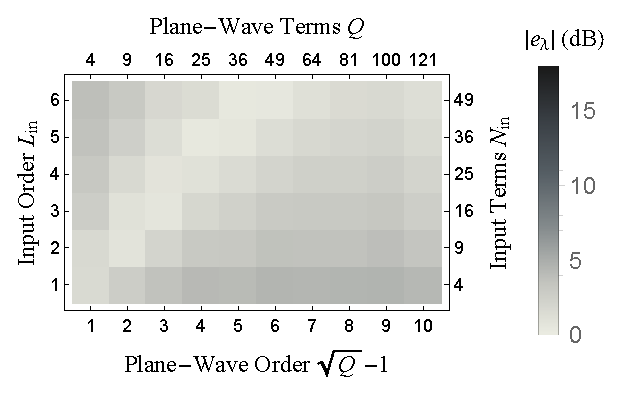
\includegraphics[width=\textwidth]{07_characterization_extrapolation/figures/audibleEnergy_order_pwt-bf.eps}
        		\caption{Level error $e_\lambda$ -- beamforming}
        		\label{fig:07_Characterization_Extrapolation:Level_Order:PWT-bf}
    	\end{subfigure}
	\hfill
    	\begin{subfigure}[b]{0.49\textwidth}
        		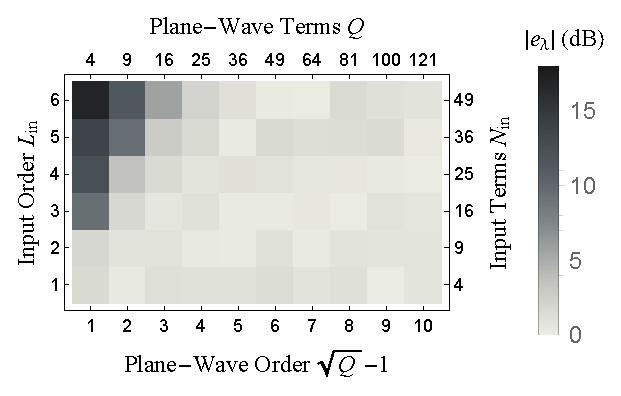
\includegraphics[width=\textwidth]{07_characterization_extrapolation/figures/audibleEnergy_order_pwt-pinv.eps}
        		\caption{Level error $e_\lambda$  -- pseudoinversion}
        		\label{fig:07_Characterization_Extrapolation:Level_Order:PWT-pinv}
    	\end{subfigure}
	
	\vspace{0.5cm}
	\begin{subfigure}[b]{0.49\textwidth}
        		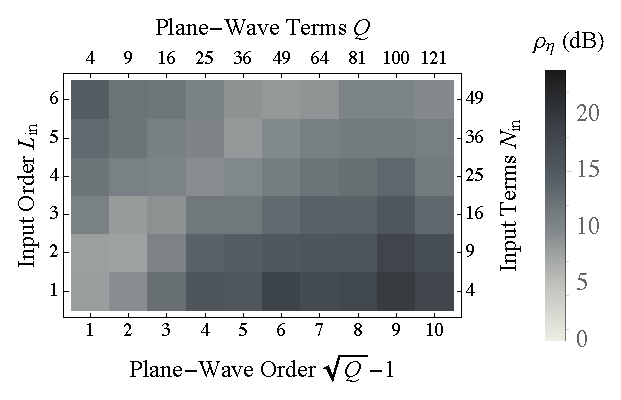
\includegraphics[width=\textwidth]{07_characterization_extrapolation/figures/scharer2009_order_pwt-bf.eps}
        		\caption{Spectral error $\rho_\eta$ -- beamforming}
        		\label{fig:07_Characterization_Extrapolation:Spectral_Order:PWT-bf}
    	\end{subfigure}
	\hfill
    	\begin{subfigure}[b]{0.49\textwidth}
        		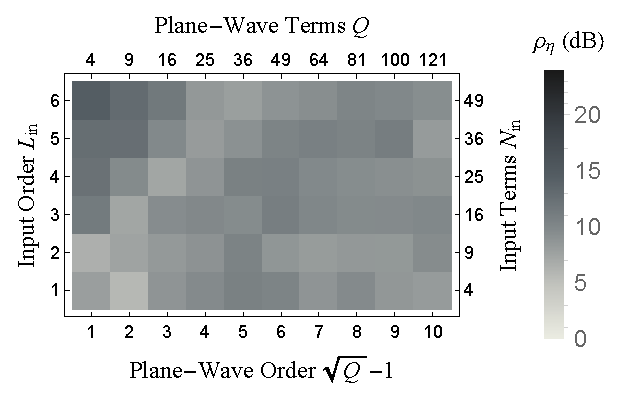
\includegraphics[width=\textwidth]{07_characterization_extrapolation/figures/scharer2009_order_pwt-pinv.eps}
        		\caption{Spectral error $\rho_\eta$ -- pseudoinversion}
        		\label{fig:07_Characterization_Extrapolation:Spectral_Order:PWT-pinv}
    	\end{subfigure}
	
	\caption[Dependence of errors on plane-wave terms and ambisonics input order.]{
	Dependence of errors on $Q$ and ambisonics input order $L_\text{in}$ (continued on p.~\pageref{fig:07_Characterization_Extrapolation:PWT_Order_Dependence:contd}).}
	\label{fig:07_Characterization_Extrapolation:PWT_Order_Dependence}
\end{figure*}

From \figref{fig:07_Characterization_Extrapolation:Level_Order:PWT-pinv}, we see a similar region of small errors, but it is less pronounced, since for $Q > N_\text{in}$ (bottom right corner of the plot), the errors are also small.
However, we note that a region of very large errors exists where $Q < N_\text{in}$ (top left corner).
This suggests that, for the pseudoinversion method, it is advantageous to have $Q \geq N_\text{in}$;
i.e., to have at least as many plane-wave terms as ambisonics signals.

The spectral errors (as defined in \secref{sec:04_Auditory_Models:Coloration_Metrics:ABSE}) for each method are plotted in \figreftwo{fig:07_Characterization_Extrapolation:Spectral_Order:PWT-bf}{fig:07_Characterization_Extrapolation:Spectral_Order:PWT-pinv}, which show trends similar to those exhibited by the level errors discussed above.
From these plots, it is clear that only the critically-sampled condition is ideal for the beamforming method.
This is in agreement with the finding of \citet[cf.~Fig.~7]{HahnSpors2015b}: that the critical-sampling condition yields decreased coloration (compared to oversampling) when using the beamforming method.
From \figref{fig:07_Characterization_Extrapolation:Spectral_Order:PWT-pinv}, we see that both the critical-sampling and oversampling conditions yield small errors for the pseudoinversion method.
Oversampling and undersampling for the beamforming method, as well as undersampling for the pseudoinversion method, all yield significantly larger errors than other conditions.

From \figreftwo{fig:07_Characterization_Extrapolation:Localization_Order:PWT-bf}{fig:07_Characterization_Extrapolation:Localization_Order:PWT-pinv}, we see that both methods yield large localization errors (as computed with \eqnref{eq:04_Auditory_Models:Localization_Error} for the localization model described in \secref{sec:05_Proposed_Models:Localization_Model}) for undersampled conditions.
For the beamforming method, the errors are otherwise uniformly small, except at very small ambisonics orders ($L_\text{in} = 1$).
That these errors do not improve with increasing $Q$ corroborates the finding of \citet[cf.~Fig.~4]{Winter2014}: that increasing the number of plane-waves beyond critically-sampled does not improve localization when using the beamforming method.
From \figref{fig:07_Characterization_Extrapolation:Localization_Order:PWT-pinv}, we see that the pseudoinversion method appears sensitive to mismatches between $Q$ and $N_\text{in}$ given the presence of large, sporadic errors that do not follow any obvious pattern.

\begin{figure*}[t]\ContinuedFloat
	\begin{subfigure}[b]{0.49\textwidth}
        		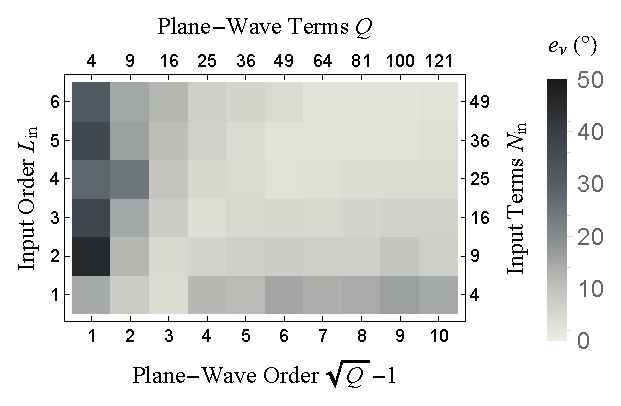
\includegraphics[width=\textwidth]{07_characterization_extrapolation/figures/tylka2017_order_pwt-bf.eps}
        		\caption{Localization error $e_\nu$ -- beamforming}
        		\label{fig:07_Characterization_Extrapolation:Localization_Order:PWT-bf}
    	\end{subfigure}
	\hfill
    	\begin{subfigure}[b]{0.49\textwidth}
        		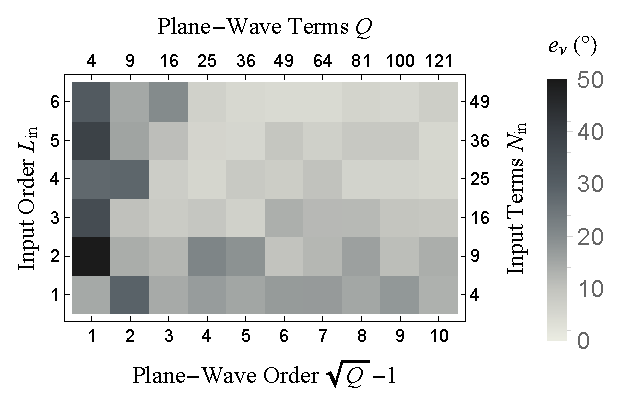
\includegraphics[width=\textwidth]{07_characterization_extrapolation/figures/tylka2017_order_pwt-pinv.eps}
        		\caption{Localization error $e_\nu$ -- pseudoinversion}
        		\label{fig:07_Characterization_Extrapolation:Localization_Order:PWT-pinv}
    	\end{subfigure}
	
	\vspace{0.5cm}
	\begin{subfigure}[b]{0.49\textwidth}
        		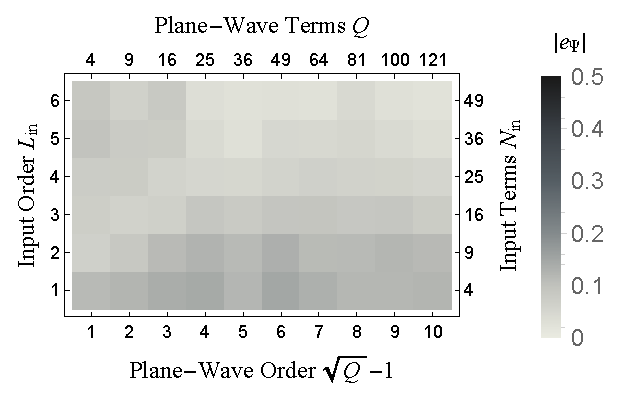
\includegraphics[width=\textwidth]{07_characterization_extrapolation/figures/merimaa2005_d_order_pwt-bf.eps}
        		\caption{Diffuseness error $e_\Psi$ -- beamforming}
        		\label{fig:07_Characterization_Extrapolation:Diffuseness_Order:PWT-bf}
    	\end{subfigure}
	\hfill
    	\begin{subfigure}[b]{0.49\textwidth}
        		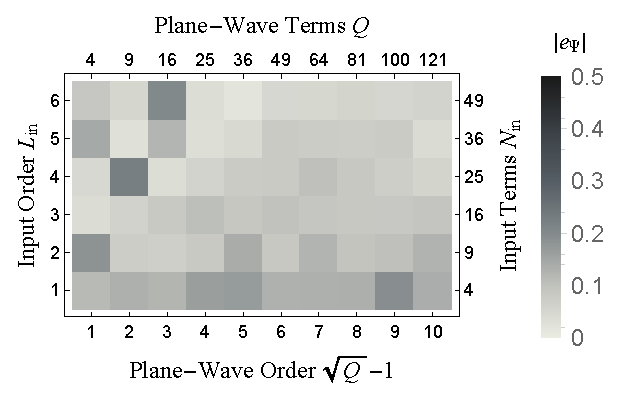
\includegraphics[width=\textwidth]{07_characterization_extrapolation/figures/merimaa2005_d_order_pwt-pinv.eps}
        		\caption{Diffuseness error $e_\Psi$ -- pseudoinversion}
        		\label{fig:07_Characterization_Extrapolation:Diffuseness_Order:PWT-pinv}
    	\end{subfigure}
	
    	\caption[]{Dependence of errors on $Q$ and ambisonics input order $L_\text{in}$ (continued from p.~\pageref{fig:07_Characterization_Extrapolation:PWT_Order_Dependence}).}
    	\label{fig:07_Characterization_Extrapolation:PWT_Order_Dependence:contd}
\end{figure*}

From the diffuseness errors (see \secref{sec:04_Auditory_Models:Diffuseness_Parameter}) plotted in \figref{fig:07_Characterization_Extrapolation:Diffuseness_Order:PWT-bf}, we see that the beamforming method only yields relatively large errors at low ambisonics orders, e.g., $L_\text{in} = 1,2$.
For the pseudoinversion method, however, we again see a sensitivity to mismatched sampling conditions, yielding relatively large errors without any discernible pattern.
Consequently, unless the plane-wave terms can be carefully chosen ahead of time for a given ambisonics order, beamforming is likely the safer method.

\section{Source azimuth dependence}\label{sec:07_Characterization_Extrapolation:Azimuth_Dependence}
In this section, we examine the effective frequency response induced by translation via each method as a function of source azimuth.
As described in \secref{sec:06_Simulation_Framework:Azimuth_Dependence}, for these simulations, we let $L_\text{in} = 4$, pick $u = 0.25$~m and $s_0 = 2.5$~m (so $\gamma = 10$), and translate to $\vec{r}_0 = (0, 0, 0)$.
Based on the findings discussed above, here we use beamforming with $Q = N_\text{in} = 25$ for the plane-wave translation method.

The induced frequency responses are plotted in \figref{fig:07_Characterization_Extrapolation:Azimuth_Dependence}.
From \figref{fig:07_Characterization_Extrapolation:Azimuth_Dependence:PWT}, we see that the plane-wave translation method introduces sporadic notches in the frequency response of the signal, which do not appear to follow any obvious pattern.
Otherwise, however, the frequency responses are largely flat for all source azimuths.
This is in agreement with the finding of \citet[cf.~Figs.~7c and 7f]{HahnSpors2015b}: that the induced frequency responses are largely flat under critically-sampled conditions, i.e., when the number of plane-wave terms matches the number of ambisonics signals.

\begin{figure*}[t]
    	\centering
    	\begin{subfigure}[b]{0.49\textwidth}
        		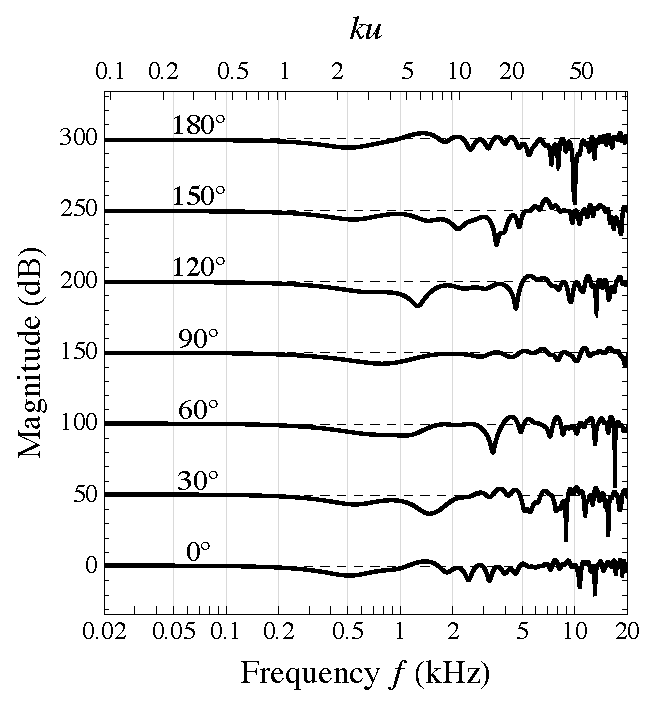
\includegraphics[width=\textwidth]{07_characterization_extrapolation/figures/sourceAz_freqResp_pwt.eps}
        		\caption{Plane-wave translation}
        		\label{fig:07_Characterization_Extrapolation:Azimuth_Dependence:PWT}
    	\end{subfigure}
	\hfill
    	\begin{subfigure}[b]{0.49\textwidth}
        		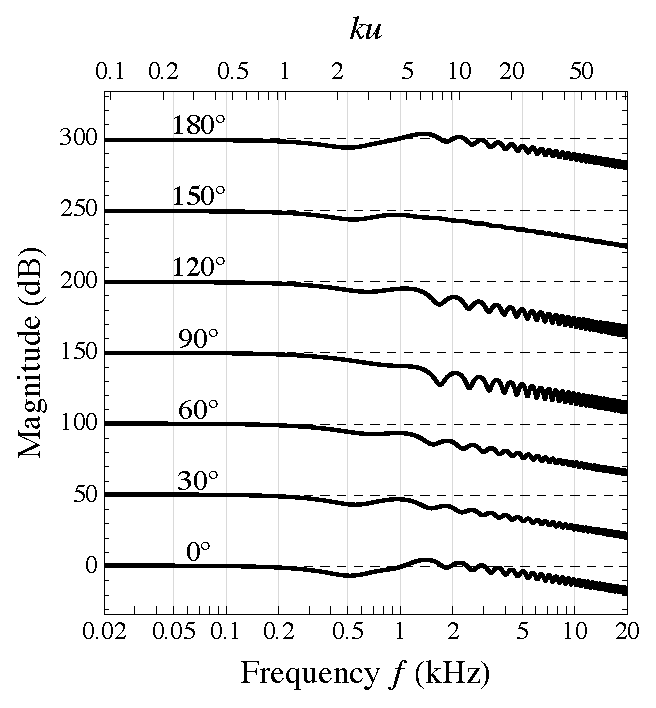
\includegraphics[width=\textwidth]{07_characterization_extrapolation/figures/sourceAz_freqResp_sre.eps}
        		\caption{Ambisonics translation}
        		\label{fig:07_Characterization_Extrapolation:Azimuth_Dependence:SRE}
    	\end{subfigure}
	
	\caption[Magnitude responses across azimuths for each extrapolation method.]{
	Magnitude responses caused by the plane-wave and ambisonics translation methods for various source azimuths.
  The bottom axes show frequency in kHz while the top axes show the nondimensional frequency $ku$ for a microphone distance of $u = 0.25$~m.
  For legibility, each frequency response is offset by $50$~dB and the responses have been artificially truncated (where needed) to not exceed $-45$~dB.}
	\label{fig:07_Characterization_Extrapolation:Azimuth_Dependence}
\end{figure*} %%NOTE%% vertical axis label is too complicated: |A0 / B0ref| or something

We also note from \figref{fig:07_Characterization_Extrapolation:Azimuth_Dependence:PWT} that the frequency response for a source azimuth of $90^\circ$ is particularly flat, which suggests that translation perpendicular to the direction of the source introduces very little spectral coloration.
This appears to contradict another finding of \citet{HahnSpors2015b}: that translation parallel to the source direction introduces less coloration than translation perpendicularly.
However, their finding was only shown for oversampled conditions, where $Q > N_\text{in}$ \citep[cf.~Fig.~7]{HahnSpors2015b}; for critically-sampled conditions (where $Q = N_\text{in}$), as considered here, the induced coloration is apparently smaller (albeit not nearly as significantly so) for perpendicular translations.

As shown in \figref{fig:07_Characterization_Extrapolation:Azimuth_Dependence:SRE}, the ambisonics translation method introduces a high-frequency roll-off, which does not depend on source azimuth.
Recall from \secref{sec:03_Navigation_Techniques:SR_Technique}, however, that the corner frequency of this roll-off does vary proportionally to $L_\text{in} / \| \vec{r}_0 - \vec{u} \|$.
Consequently, we expect the spectral coloration induced by this method to increase steadily with increasing translation distance, while the overall level will steadily decrease.

\section{Characterization and discussion}\label{sec:07_Characterization_Extrapolation:Results}
Based on our findings in \secref{sec:07_Characterization_Extrapolation:Plane-wave_Dependence}, we use beamforming with $Q = N_\text{in}$ for the plane-wave translation method in all simulations discussed below.

% Level

Level error contour plots are shown in the top panels of \figref{fig:07_Characterization_Extrapolation:Level_Spectral_Errors}.
For the plane-wave translation method (see \figref{fig:07_Characterization_Extrapolation:Level_Errors:PWT}), we see that exterior sources experience negligible level error;
interior sources, however, are reproduced approximately $6$~dB too quietly for most microphone distances.
For the ambisonics translation method (see \figref{fig:07_Characterization_Extrapolation:Level_Errors:SRE}), we see a general trend of increasing level error with microphone distance at all source distances, although exterior sources consistently experience less severe level errors than interior ones for the same $u$, and at very large $u$ and $\gamma$ (top right corner of \figref{fig:07_Characterization_Extrapolation:Level_Errors:SRE}), the errors become less severe.
The degradation in performance with increasing microphone distance is due to the high-frequency roll-off induced by the ambisonics translation filters, as discussed in \secref{sec:07_Characterization_Extrapolation:Azimuth_Dependence}, which yields a decrease in overall level.
Taken together, these results imply that a violation of the region of validity restriction (i.e., for interior sources) tends to yield a reproduced level that is significantly too low. % overall, exterior is much better; violating region of validity --> too quiet

\begin{figure*}[tbp]
    	\centering
    	\begin{subfigure}[b]{0.49\textwidth}
        		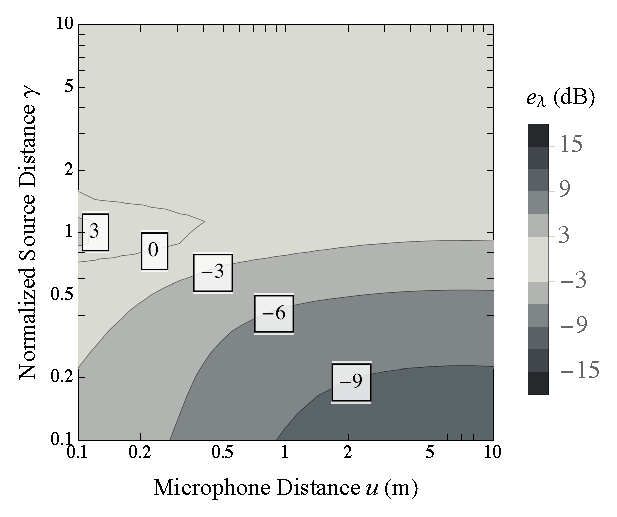
\includegraphics[width=\textwidth]{07_characterization_extrapolation/figures/audibleEnergy_contour_pwt.eps}
        		\caption{$e_\lambda$ -- plane-wave translation}
        		\label{fig:07_Characterization_Extrapolation:Level_Errors:PWT}
    	\end{subfigure}
	\hfill
    	\begin{subfigure}[b]{0.49\textwidth}
        		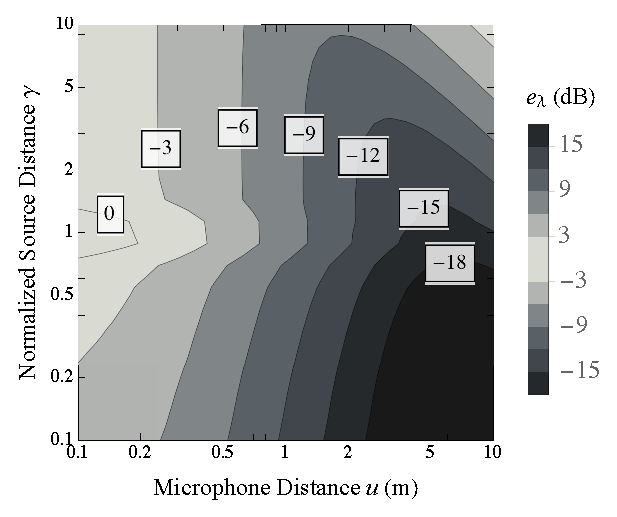
\includegraphics[width=\textwidth]{07_characterization_extrapolation/figures/audibleEnergy_contour_sre.eps}
        		\caption{$e_\lambda$ -- ambisonics translation}
        		\label{fig:07_Characterization_Extrapolation:Level_Errors:SRE}
    	\end{subfigure}
	
	\vspace{0.5cm}
	\begin{subfigure}[b]{0.49\textwidth}
        		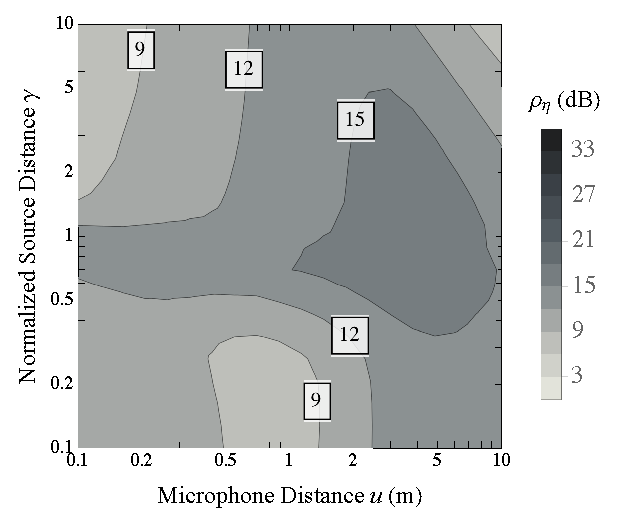
\includegraphics[width=\textwidth]{07_characterization_extrapolation/figures/scharer2009_contour_pwt.eps}
        		\caption{$\rho_\eta$ -- plane-wave translation}
        		\label{fig:07_Characterization_Extrapolation:Spectral_Errors:PWT}
    	\end{subfigure}
	\hfill
    	\begin{subfigure}[b]{0.49\textwidth}
        		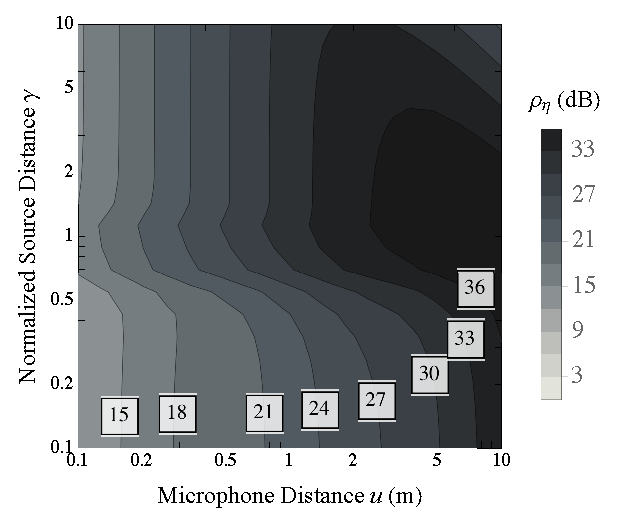
\includegraphics[width=\textwidth]{07_characterization_extrapolation/figures/scharer2009_contour_sre.eps}
        		\caption{$\rho_\eta$ -- ambisonics translation}
        		\label{fig:07_Characterization_Extrapolation:Spectral_Errors:SRE}
    	\end{subfigure}
	
    	\caption[Level and coloration contour plots for each extrapolation method.]{
	Level errors $e_\lambda$ (top panels) and spectral errors $\rho_\eta$ (bottom) for microphone distance $u$ and normalized source distance $\gamma$.
  Contour lines are drawn every $3$~dB.}
    	\label{fig:07_Characterization_Extrapolation:Level_Spectral_Errors}
\end{figure*}

% Coloration

In the bottom panels of \figref{fig:07_Characterization_Extrapolation:Level_Spectral_Errors}, we plot the spectral errors incurred by both methods.
The plane-wave translation method does not appear to exhibit any clear trend (see \figref{fig:07_Characterization_Extrapolation:Spectral_Errors:PWT}), although we do see that, for any given microphone distance, the greatest spectral errors occur for source distances around $\gamma = 1$.
Furthermore, this method tends to experience the largest spectral error ($\rho_\eta > 15$~dB) at large microphone distances ($u > 1$~m) with $\gamma \sim 1$.
Additionally, there are two regions of low error: 1) at very small microphone distances with very far-field sources (top left corner of \figref{fig:07_Characterization_Extrapolation:Spectral_Errors:PWT}) and 2) for microphone distances around $u \approx 1$~m with far interior sources ($\gamma < 0.3$).

As shown in \figref{fig:07_Characterization_Extrapolation:Spectral_Errors:SRE}, the ambisonics translation method exhibits similar behavior in terms of spectral error as it does for level errors:
in this plot, we again see a clear trend of increasing error with microphone distance (again due to the high-frequency roll-off), with the exception of a region of slightly less severe errors at very large $u$ and $\gamma$.
However, in this case, interior sources experience approximately $6$~dB less spectral error than corresponding exterior ones (for a fixed $u$).

% Localization

From \figref{fig:07_Characterization_Extrapolation:Localization_Errors:PWT}, we see that the plane-wave translation method introduces very small localization errors for exterior sources.
This is somewhat intuitive, since as $\gamma$ increases, the source appears more like a plane-wave source, which should be natural to reproduce using the plane-wave translation method.
The ambisonics translation method, however, is only accurate at very small microphone distances with very far exterior sources (as shown in the top left corner of \figref{fig:07_Characterization_Extrapolation:Localization_Errors:SRE}).
Otherwise, for exterior sources, the errors incurred by the ambisonics translation method increase steadily with increasing microphone distance.
Additionally, both methods yield large errors at all microphone distances for interior sources with approximately $0.3 < \gamma < 1$, as well as at very small $u$ and $\gamma$ (bottom left corners of both \figreftwo{fig:07_Characterization_Extrapolation:Localization_Errors:PWT}{fig:07_Characterization_Extrapolation:Localization_Errors:SRE}).
That this behavior is common to both methods implies that it is the violation of the region of validity restriction which causes these extremely large localization errors. % the band of large errors as well as the bottom left corner are common to both --> inherent to region of validity violation

\begin{figure*}[tbp]
    	\centering
    	\begin{subfigure}[b]{0.49\textwidth}
        		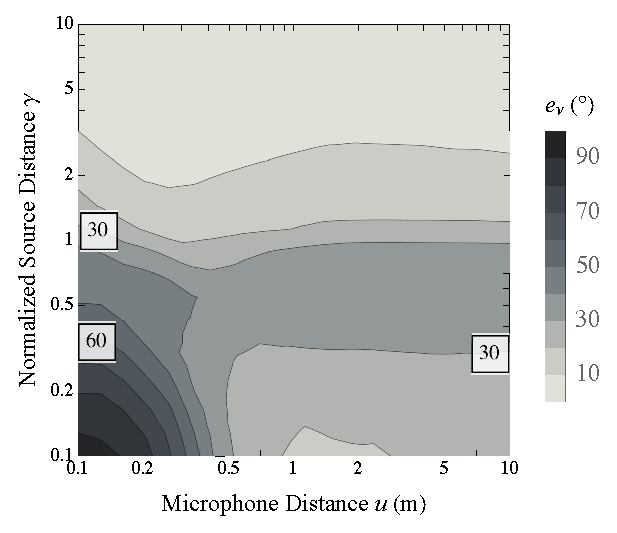
\includegraphics[width=\textwidth]{07_characterization_extrapolation/figures/tylka2017_contour_pwt.eps}
        		\caption{$e_\nu$ -- plane-wave translation}
        		\label{fig:07_Characterization_Extrapolation:Localization_Errors:PWT}
    	\end{subfigure}
	\hfill
    	\begin{subfigure}[b]{0.49\textwidth}
        		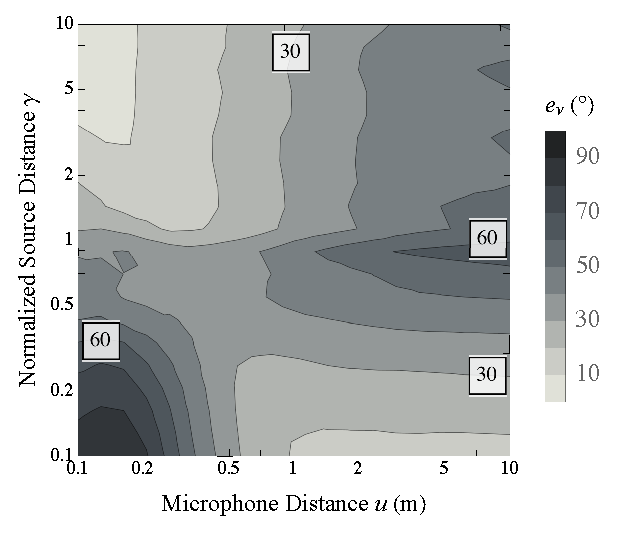
\includegraphics[width=\textwidth]{07_characterization_extrapolation/figures/tylka2017_contour_sre.eps}
        		\caption{$e_\nu$ -- ambisonics translation}
        		\label{fig:07_Characterization_Extrapolation:Localization_Errors:SRE}
    	\end{subfigure}
	
	\vspace{0.5cm}
	\begin{subfigure}[b]{0.49\textwidth}
        		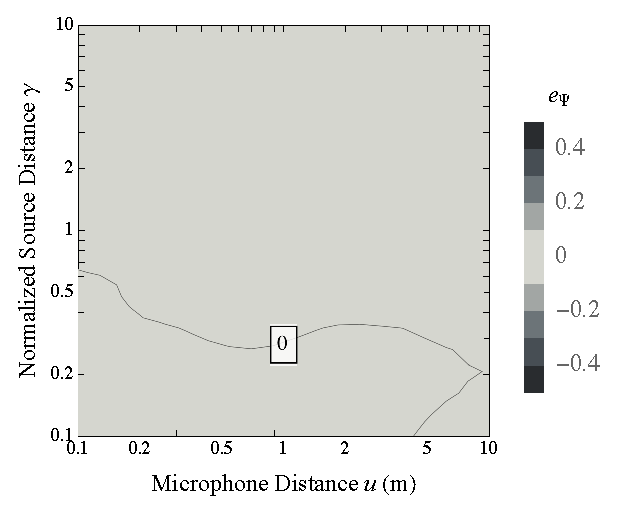
\includegraphics[width=\textwidth]{07_characterization_extrapolation/figures/merimaa2005_d_contour_pwt.eps}
        		\caption{$e_\Psi$ -- plane-wave translation}
        		\label{fig:07_Characterization_Extrapolation:Diffuseness_Errors:PWT}
    	\end{subfigure}
	\hfill
    	\begin{subfigure}[b]{0.49\textwidth}
        		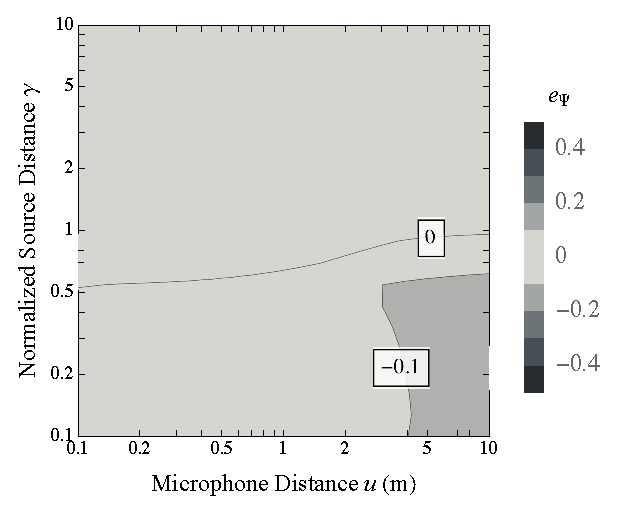
\includegraphics[width=\textwidth]{07_characterization_extrapolation/figures/merimaa2005_d_contour_sre.eps}
        		\caption{$e_\Psi$ -- ambisonics translation}
        		\label{fig:07_Characterization_Extrapolation:Diffuseness_Errors:SRE}
    	\end{subfigure}
	
    	\caption[Localization and diffuseness contour plots for each extrapolation method.]{
	Localization errors $e_\nu$ (top panels) and diffuseness errors $e_\Psi$ (bottom) for microphone distance $u$ and normalized source distance $\gamma$.
  Localization error contour lines are drawn every $10^\circ$; diffuseness error contour lines are drawn in increments of $0.1$.}
    	\label{fig:07_Characterization_Extrapolation:Localization_Diffuseness_Errors}
\end{figure*}

% Diffuseness

As shown in the bottom panels of \figref{fig:07_Characterization_Extrapolation:Localization_Diffuseness_Errors}, both methods achieve nearly zero diffuseness errors, although the ambisonics translation method exhibits a region of minor errors ($e_\Psi \approx -0.1$) for interior sources at large microphone distances (bottom right corner of \figref{fig:07_Characterization_Extrapolation:Diffuseness_Errors:SRE}).

%% Order Dependence %%
\subsection{Order dependence}
In \figref{fig:07_Characterization_Extrapolation:Order_Errors}, we plot errors for each metric and for both methods as functions of microphone distance $u$ for a fixed source distance of $s_0 = 1$~m and for several input ambisonics orders $L_\text{in}$ (with matching $Q = N_\text{in} = (L_\text{in} + 1)^2$ for the plane-wave translation method).

From \figref{fig:07_Characterization_Extrapolation:Level_Errors:Order}, we see that, in terms of level errors, increasing the ambisonics input order tends to improve performance, albeit only marginally.
Additionally, the performance of both methods degrades with increasing microphone distance, with exterior sources (where $u < s_0 = 1$~m) exhibiting significantly less severe errors than interior ones (where $u > s_0$).
Furthermore, all of these curves exhibit a ``knee'' at $u = 1$~m, where the curves experience a qualitative change in behavior.
In particular, the plane-wave translation method exhibits two distinct regimes on either side of $u = 1$~m: for exterior sources, the method incurs constant level errors, whereas for interior sources, the errors grow more extreme with increasing $u$.
For the ambisonics translation method, increasing $u$ tends to produce more extreme errors overall, and the errors grow more rapidly in the interior source regime than in the exterior source regime.
Only the plane-wave translation method with exterior sources exhibits negligible level errors ($\sim1$~dB), which is a consequence of our choice to match the number of plane-wave terms, $Q$, to the number of ambisonics signals, $N_\text{in} = (L_\text{in} + 1)^2$.

\begin{figure*}[t]
    	\centering
	\begin{subfigure}[b]{0.49\textwidth}
        		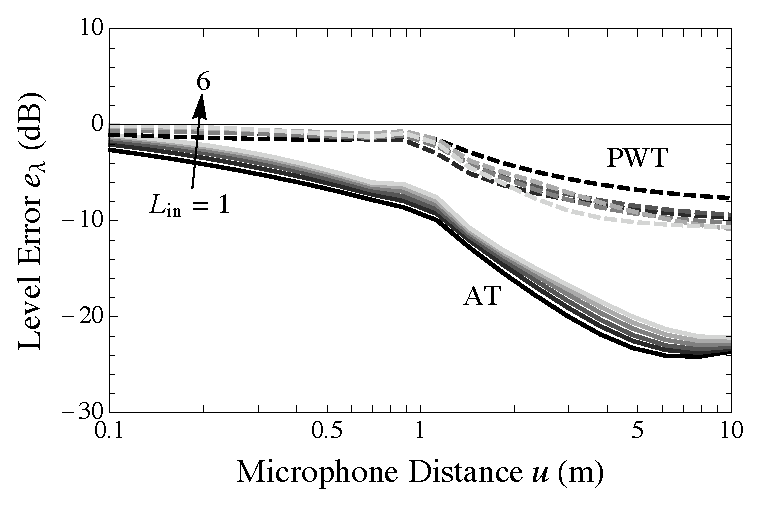
\includegraphics[width=\textwidth]{07_characterization_extrapolation/figures/audibleEnergy_order.eps}
        		\caption{Level errors $e_\lambda$}
        		\label{fig:07_Characterization_Extrapolation:Level_Errors:Order}
    	\end{subfigure}
	\hfill
    	\begin{subfigure}[b]{0.49\textwidth}
        		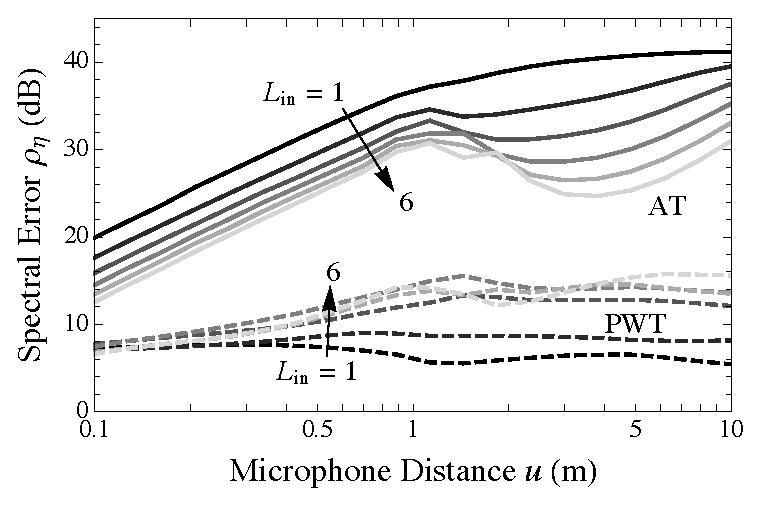
\includegraphics[width=\textwidth]{07_characterization_extrapolation/figures/scharer2009_order.eps}
        		\caption{Spectral errors $\rho_\eta$}
        		\label{fig:07_Characterization_Extrapolation:Spectral_Errors:Order}
    	\end{subfigure}
	
	\vspace{0.5cm}
	\begin{subfigure}[b]{0.49\textwidth}
        		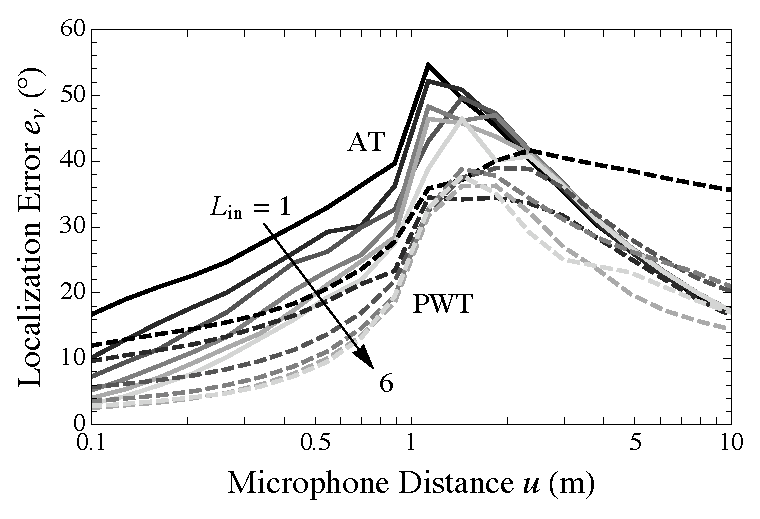
\includegraphics[width=\textwidth]{07_characterization_extrapolation/figures/tylka2017_order.eps}
        		\caption{Localization errors $e_\nu$}
		\label{fig:07_Characterization_Extrapolation:Localization_Errors:Order}
    	\end{subfigure}
	\hfill
    	\begin{subfigure}[b]{0.49\textwidth}
        		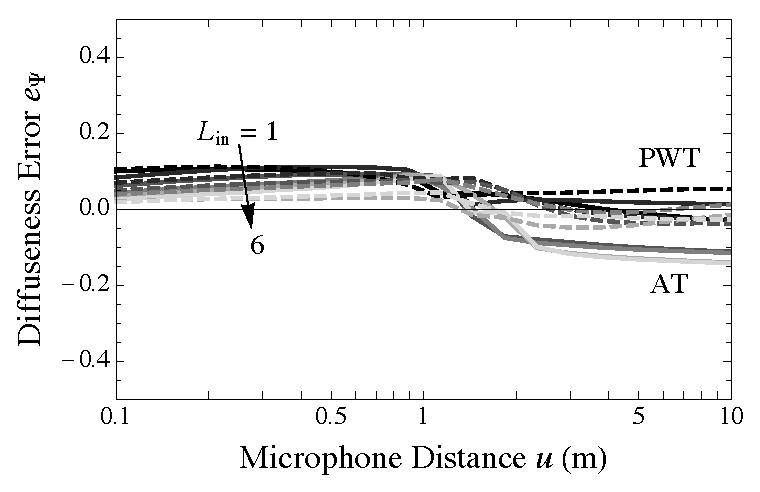
\includegraphics[width=\textwidth]{07_characterization_extrapolation/figures/merimaa2005_d_order.eps}
        		\caption{Diffuseness errors $e_\Psi$}
		\label{fig:07_Characterization_Extrapolation:Diffuseness_Errors:Order}
    	\end{subfigure}
	
    	\caption[Order dependence plots for each extrapolation method.]{
	Errors for various microphone distances $u$ with a fixed source distance $s_0 = 1$~m.
	Errors are plotted for the ambisonics translation method (solid curves, labeled ``AT'') and the plane-wave translation method (dashed curves, labeled ``PWT'').
	For each method, six input ambisonics orders are shown: $L_\textrm{in} = 1$ (black) to $L_\textrm{in} = 6$ (lightest gray).}
    	\label{fig:07_Characterization_Extrapolation:Order_Errors}
\end{figure*}

From \figref{fig:07_Characterization_Extrapolation:Spectral_Errors:Order}, we again see that increasing the ambisonics order $L_\text{in}$ yields an improvement in performance (i.e., a decrease in spectral errors) for the ambisonics translation method.
Here again we note two distinct regimes for this method on either side of $u = 1$~m with a transition region where the behavior changes.
Additionally, within each regime, the errors again increase monotonically with increasing $u$.
However, unlike with level errors, we now see a more rapid (but still monotonic) increase in error for \textit{exterior} sources ($u < 1$~m), while the more gradual performance degradation occurs for \textit{interior} sources ($u > 1$~m).
For the plane-wave translation method, we see that increasing $L_\text{in}$ yields an \textit{increase} in spectral error, and that this increase in error is more severe for interior sources than for exterior ones.
This suggests a penalty from violating the region of validity restriction that is particular to the plane-wave translation method: that a larger ambisonics input order incurs more spectral coloration.

As shown in \figref{fig:07_Characterization_Extrapolation:Localization_Errors:Order}, the localization errors for both methods tend to improve with increasing $L_\text{in}$, and the existence of two regimes on either side of $u = 1$~m is evident.
For exterior sources ($u < 1$~m), the errors improve with decreasing $u$, whereas for interior sources ($u > 1$~m), the opposite is true: the errors improve with \textit{increasing} $u$.
Evidently, a microphone distance of $u \approx s_0$ (i.e., $\gamma \approx 1$) yields the most extreme errors.
Overall, the ambisonics translation method tends to perform worse than the plane-wave translation method (except at very large $u$ and $L_\text{in} = 1$) and the errors for both methods are typically smaller for exterior sources than for interior ones.

It is worth noting that by construction, since $s_0$ is fixed, as $u$ increases beyond $1$~m, more of the navigable region (see \figref{fig:06_Simulation_Framework:Point_Geometry}) becomes valid for translation.
For instance, with $u = 10$~m and $s_0 = 1$~m, the listener can navigate approximately $9$~m away from the microphone and still remain inside its region of validity.
This explains in part the improvement with increasing $u$ seen for $u > 1$~m, since, on average, more of the navigable region is valid.
That is, when averaging errors over the entire navigable region, a smaller fraction of that region will actually be in violation of the region of validity restriction.

Finally, as shown in \figref{fig:07_Characterization_Extrapolation:Diffuseness_Errors:Order}, both methods achieve small diffuseness errors, and generally, increasing $L_\text{in}$ improves the performance for exterior sources.
Again we see a transition between regimes occurring at $u \approx 1$~m.

\section{Conclusions}\label{sec:07_Characterization_Extrapolation:Conclusions}
In this chapter, we presented the results of numerical simulations conducted in order to characterize and compare the performance of the plane-wave and ambisonics translation methods.
Following the simulation framework laid out in \chapref{chap:06_Simulation_Framework}, we simulated simple incident sound fields consisting of a single microphone and a single point-source, varying source distance and azimuth, as well as microphone distance and listener position.
First, in \secref{sec:07_Characterization_Extrapolation:Plane-wave_Dependence}, we determined suitable parameters for the plane-wave translation method, comparing the beamforming and pseudoinversion methods for computing the plane-wave decomposition and varying both the ambisonics input order and the number of plane-wave terms.
We then explored, in \secref{sec:07_Characterization_Extrapolation:Azimuth_Dependence}, basic properties of each method by computing the effective frequency responses induced by the plane-wave and ambisonics translation methods across source azimuths.
Finally, in \secref{sec:07_Characterization_Extrapolation:Results}, we conducted a more comprehensive analysis of both methods in terms of the metrics enumerated in \secref{sec:06_Simulation_Framework:Metrics} for sound level, spectral coloration, source localization, and diffuseness.

The analyses presented in this chapter yielded the following major findings:
\begin{itemize}
\item for the plane-wave translation method, a clear advantage exists to using the beamforming plane-wave decomposition method (see \eqnref{eq:02_Acoustical_Theory:A2mu}) and matching the number of ambisonics signals, $N$, to the number of plane-wave terms, $Q$;%
\footnote{All subsequent findings relate to this implementation of the plane-wave translation method: beamforming with matched $Q = N$.}
%\item the pseudoinversion plane-wave decomposition method (see \eqnref{eq:02_Acoustical_Theory:A2mu_Pinv}) exhibited a similar advantage, as well as an advantage to ``oversampling'' directions by taking $Q > N$, although this method also appeared more sensitive to mismatches than the beamforming method;
\item the frequency responses induced by the plane-wave translation method are largely flat but with sporadic notches while those induced by the ambisonics translation method exhibit a consistent low-pass-like roll-off of high-frequency energy, but both methods appear largely insensitive to source azimuth;
\item the ambisonics translation method incurs significant errors in both level and coloration at all source distances which, overall, increase steadily with microphone distance;
\item for exterior sources, the plane-wave translation method achieves a high degree of accuracy in both level and localization;
\item for interior sources, where the region of validity restriction is violated, both methods incur significant errors in both level and localization; and
\item more generally, both methods tend to exhibit two distinct regimes of behavior for exterior and interior sources, with a transition region between the two, and the performance for interior sources is often degraded compared to that for exterior sources.
\end{itemize}
Additionally, results showed that increasing the ambisonics order tends to uniformly improve the performance of both methods, with the exception of the spectral errors incurred by the plane-wave translation method.

Due to the extremely large level and coloration errors incurred by the ambisonics translation method, the plane-wave translation method is likely the only viable method for most applications with practical translation distances (e.g., $u > 0.5$~m).
This method is particularly well-suited for exterior sources, but its performance degrades significantly, in terms of localization in particular, once the region of validity restriction is violated.
The remaining challenge for this method is the introduction of significant spectral errors ($\rho_\eta > 10$~dB) over all microphone and source distances.
Consequently, future improvements to this method should attempt to correct this coloration, perhaps parametrically based on source direction.

As demonstrated in this chapter, the performance of linear extrapolation-based navigational methods is significantly impaired by the presence of near-field sources.
Consequently, parametric and interpolation-based approaches have been developed that aim to extend navigation beyond such near-field sources while maintaining acceptable performance.
In the following chapters, we characterize and compare the performance of several such methods:
in \chapref{chap:08_Proposed_Method}, we propose a parametric interpolation method and demonstrate its improvement over a benchmark linear interpolation method and,
in \chapref{chap:09_Thiergart_Comparison}, we perform a similar analysis of an existing parametric interpolation method.

\section*{Acknowledgements}
This work is a significantly updated version of a paper originally presented by \citet{TylkaChoueiri2015} at the 139\textsuperscript{th} Convention of the Audio Engineering Society.
The analysis presented here was originally submitted by \citet{TylkaChoueiri2019c} to \textit{The Journal of the Audio Engineering Society}.